\documentclass[11pt]{article}
\usepackage[margin=1in]{geometry}
\usepackage{booktabs}
\usepackage{threeparttable}
\usepackage{graphicx}
\usepackage{float}
\usepackage{amsmath}
\usepackage{hyperref}

\title{Manufactured Housing Classification: Model Performance and Validation}
\date{\today}

\begin{document}

\maketitle

\section{Overview}

This document evaluates a Light Gradient Boosting Machine (LightGBM) classifier designed to identify manufactured home loans in HMDA data from 1990-2003, a period when property type information was not systematically collected. The classifier addresses a critical missing data problem that affects research on subprime lending and housing policy during this key historical period.

\subsection{The Missing Data Problem}

Prior to 2004, the Home Mortgage Disclosure Act (HMDA) did not require lenders to report property type information, creating a substantial gap in our understanding of manufactured home lending patterns during the 1990s and early 2000s. This period coincides with significant expansion in subprime lending and represents a crucial era for understanding housing finance disparities. The lack of property type data prevents researchers from analyzing manufactured home lending patterns, geographic concentration, and borrower characteristics during this formative period.

\subsection{Light GBM Methodology}

I employ a Light Gradient Boosting Machine, a tree-based ensemble method similar to a random forest, that excels at handling mixed-type data with categorical and continuous features. The model is trained on HMDA data from 2004-2013 (when property type was reported) and validated on 2014-2017 data. Key advantages of LightGBM include: efficient handling of categorical variables without extensive preprocessing, robust performance with missing values and class imbalance, and the ability to capture complex interactions between features.

The model uses loan characteristics (amount, loan-to-income ratio), geographic features (rural status, tract-level housing composition), lender attributes (average loan size, lending volume), and borrower demographics to predict manufactured home status.

\section{Training Data Characteristics}

Table \ref{tab:sum-stats} presents descriptive statistics for the key features used in the classification model separately for site-built and mobile homes in the training data (2004-2013). There are stark differences in loans for manufactured and site-built homes.

\input{results/tables/sum-stats.tex}

Several patterns emerge from the training data that inform the classifier's predictions. Manufactured home loans average significantly smaller amounts (\$75,000 vs \$209,000 for site-built homes) and serve borrowers with lower incomes (\$51,000 vs \$98,000). Geographic concentration is pronounced, with manufactured home loans occurring disproportionately in rural areas and census tracts with higher shares of mobile homes. These stark differences suggest that a classifier based on loan-level characteristics will be able to identify manufactured home loans.

\section{Model Performance and Validation}

\subsection{Classification Metrics}

Table \ref{tab:model_metrics} reports performance metrics across training, validation, and test periods. To understand these results, it's helpful to think of the classification task as distinguishing between manufactured home loans and site-built home loans in historical data where this information was not originally recorded.

\input{results/tables/model_metrics.tex}

Model Discrimination Ability: The AUC (Area Under the Curve) measures how well the model distinguishes between the two types of loans, where 0.5 represents random guessing and 1.0 represents perfect classification. The model achieves excellent discrimination across all time periods, with AUC values of 0.987, 0.985, and 0.978 for training, validation, and test periods respectively. These high values indicate the model reliably separates manufactured from site-built home loans.

Overall Accuracy: The model correctly classifies over 91\% of all loans across time periods. While this seems high, it's important to note that manufactured homes represent a small fraction of total loans, so high overall accuracy doesn't guarantee good performance on the minority class of interest.

Identifying Manufactured Home Loans: Sensitivity (also called recall) measures what percentage of actual manufactured home loans the model successfully identifies. This is crucial for research purposes—missing manufactured home loans would bias any subsequent analysis. The model demonstrates strong performance here, correctly identifying 95.1\% of manufactured home loans in training data, 94.1\% in validation, and 92.6\% in the test period.

Avoiding False Positives: Precision indicates that among loans predicted to be manufactured homes, what percentage actually are manufactured homes. The model achieves precision of 26.4\%, 25.2\%, and 21.6\% across the three periods. While this may seem low, it reflects the challenge of the heavily imbalanced dataset where manufactured homes constitute a small fraction of total loans. Put differently, for every four loans the model identifies as manufactured homes, approximately one is actually a manufactured home.

Balanced Performance: The F1 score provides a single measure balancing precision and sensitivity, which is particularly useful for imbalanced classification problems like this one. F1 scores of 0.413, 0.397, and 0.350 across periods indicate reasonable performance given the class imbalance challenge.
The modest decline in performance from training to test periods (AUC drops from 0.987 to 0.978, F1 from 0.413 to 0.350) suggests some temporal drift but indicates the model remains robust for historical prediction. Most importantly for research applications, the model maintains high sensitivity above 92\% across all periods, meaning it successfully captures the vast majority of manufactured home loans while maintaining reasonable control over false positives.

\subsection{The Model is Not Using Only The Loan Amounts}

One concern with the classifier is that it may rely too heavily on the amount of the loan to distinguish between site-built and manufactured homes. Such a reliance would cause a problem in the historical analysis: loan amounts have changed over time and may not be comparable across periods. Moreover, loan amounts are a key outcome of interest, and comparing effects on loan amounts separately for manufactured and site-built homes would be problematic if the model is using loan amounts to distinguish between the two.

I investigate this concern by plotting the density of loan amounts for manufactured and site-built homes in the imputed dataset. Figure \ref{fig:loan_amounts} shows the distribution of loan amounts for manufactured homes (in blue) and site-built homes (in orange). The two distributions overlap significantly, especially in the critical interval between \$60,000 and \$100,000, indicating that the classifier is not relying solely on loan amounts to distinguish between the two property types.

\begin{figure}[htbp]
    \centering
    \caption{Loan Amounts by Imputed Property Type}\label{fig:loan_amounts}
    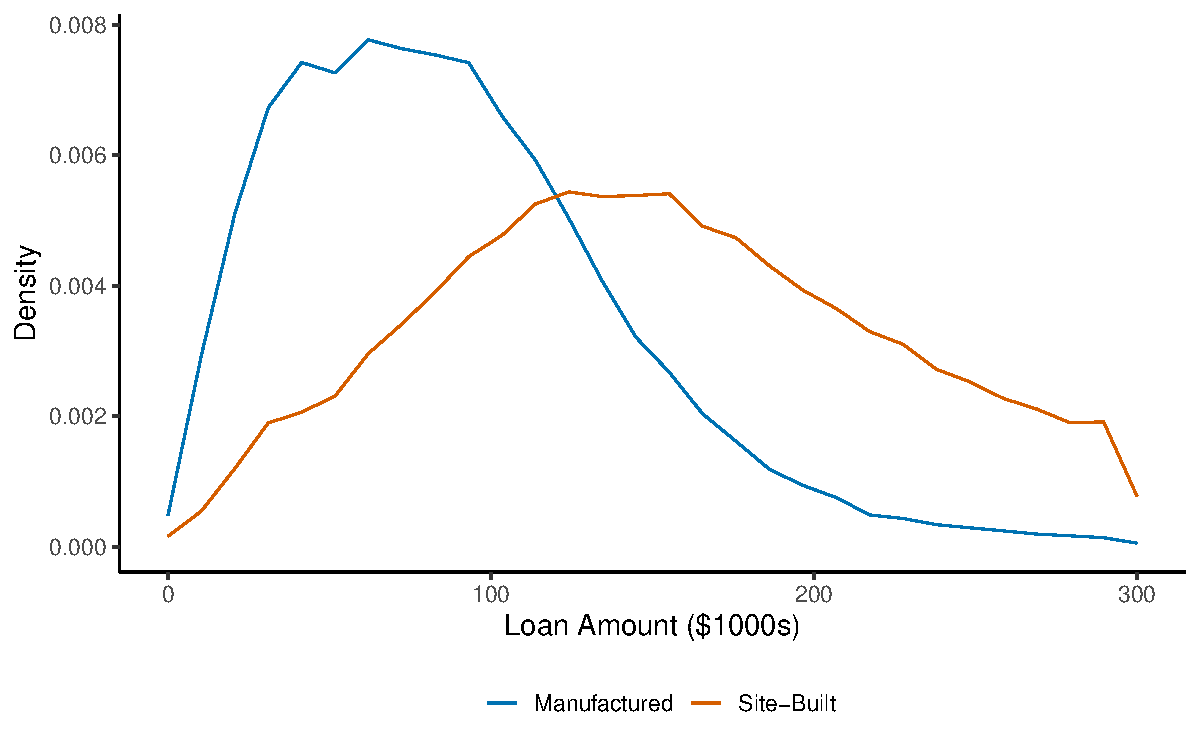
\includegraphics[width=0.8\textwidth]{results/plots/loan_amounts_by_imputed_type.pdf}
    \begin{minipage}{0.8\textwidth}
    \begin{flushleft}
        \begin{footnotesize}
    \emph{Notes:  }Density of loan amounts for manufactured homes (blue) and site-built homes (orange) in the imputed HMDA data (1990 - 2003). Loans exceeding \$300,000 are excluded for clarity.
        \end{footnotesize}
    \end{flushleft}
    \end{minipage}
\end{figure}

\subsection{External Validation Against Census Data}

Figure \ref{fig:orig_place} compares the model's predictions for 1993-2003 against independent Census data on manufactured home placements. While the model successfully captures the decline in manufactured housing that begin in 1999, the decline in originations lags that of placements. In part, this reflects the fact that mortgage originations also depend on the stock of existing homes, not just new placements.

\begin{figure}[htbp]
    \centering
    \caption{Comparison of Imputed Originations and Census Placements}
    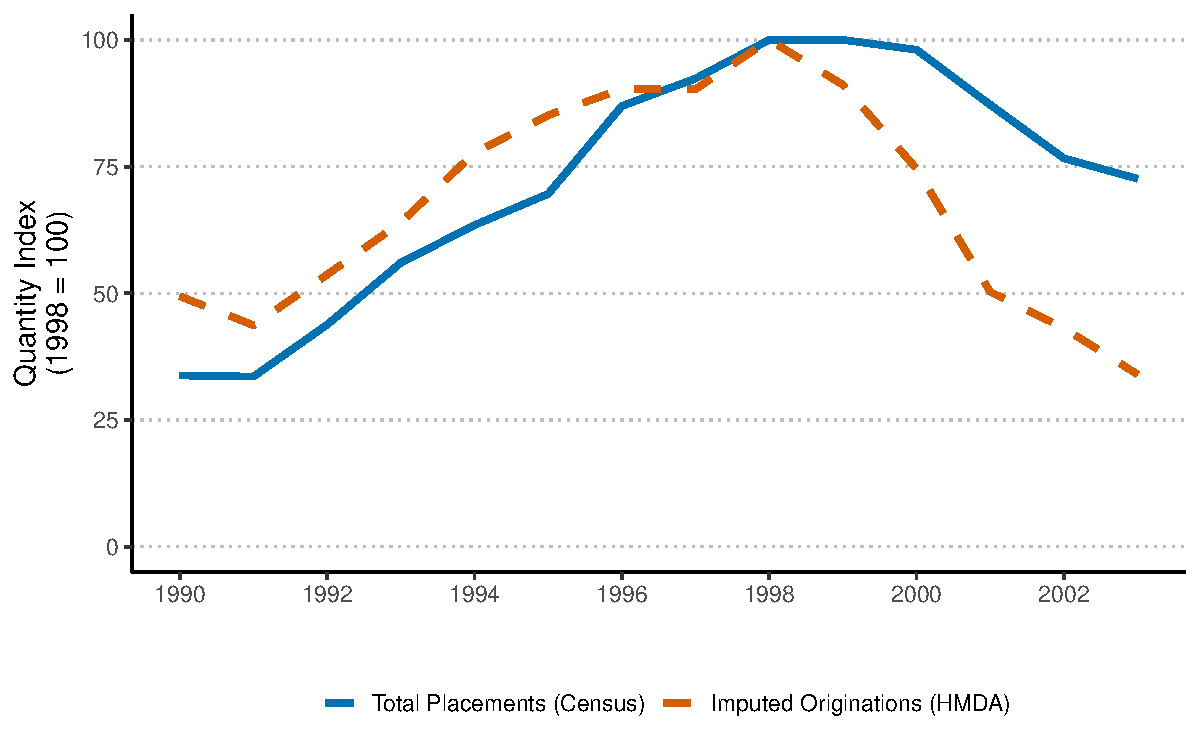
\includegraphics[width=0.8\textwidth]{results/plots/orig_tot-place_tot.pdf}
    \begin{minipage}{0.8\textwidth}
    \begin{flushleft}
        \begin{footnotesize}
    \emph{Notes:  }Census placements represent new manufactured homes placed for residential use. HMDA originations represent predicted manufactured home loan originations from the classifier. Both series indexed to 1998=100.
        \end{footnotesize}
    \end{flushleft}
    \end{minipage}
    \label{fig:orig_place}
\end{figure}

\subsection{Quantitative Validation}

Table \ref{orig-place-reg} presents a state-level regression relating total imputed originations to total Census placements. The two variable are highly correlated with an elasticity of roughly 0.7. 

\input{results/tables/orig_tot-place_tot.tex}

The estimated elasticity of 0.89 indicates that states with higher manufactured home placement rates also show correspondingly higher rates of imputed originations in the HMDA predictions. The high R-squared (0.72) demonstrates that Census placement data explains substantial variation in the predictions at the state level, providing quantitative validation of the classification approach.

\section{Implications and Limitations}

This classification enables analysis of manufactured home lending patterns during the critical 1990-2003 period, when subprime lending expanded rapidly. The model's consistent performance and external validation against Census data provide confidence for historical analysis. However, users should note the model's precision limitations (around 65\%) and the possibility of systematic biases in time periods or geographic areas with substantially different lending patterns than the training period.

The methodology could be extended to other missing data problems in financial datasets and provides a template for handling systematic data gaps in historical mortgage research.

\end{document}